\frame
{
  \frametitle{ Event Forecasting with Pattern Markov
 	Chains \cite{alevizos2017event} }
	\framesubtitle{overview}
  \begin{itemize}[]
  	\item<1-> The model handles a single input stream $s_i$ of events.
  	\item<1-> The event stream $s_i$ is assumed to be generated by $m$-order Markov source.
  \item<1-> The  event pattern $\mathcal{P}$ is defined in the form of regular expressions over a finite set of event types $\Sigma$.

  \item<1-> A probabilistic model provides online forecasting reports when the $\mathcal{P}$ is expected to be completed in future. 
   
  \end{itemize}
}

\frame
{
	\frametitle{Event Forecasting with Pattern Markov
		Chains  }
	\framesubtitle{ How does it work?}
		\begin{itemize}
		\item<only@1> The pattern $\mathcal{P}=a ; d ; c$ is converted to deterministic finite automaton ($DFA$) with $\Sigma=\{a,b,c,d\}$. 
		
 \begin{figure}[ht]
	\begin{center}
		
	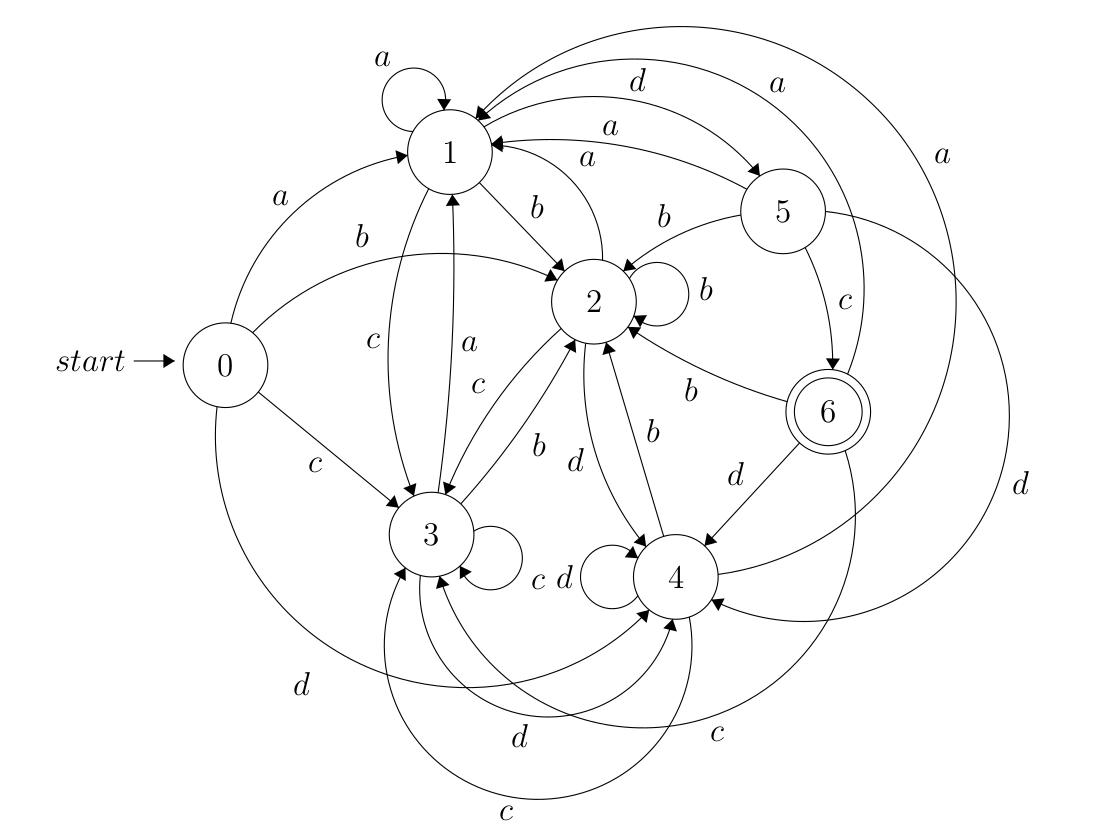
\includegraphics[width=\linewidth,height=.6\textheight,left]{figures/new/dfa.png}\linebreak
$Q=\{0,1,2,3,4,5,6\}$ for  $m=1$
\end{center}
%\caption[]{}
\end{figure}

	
			\end{itemize}
}

\frame
{
	\frametitle{Event Forecasting with Pattern Markov
		Chains}
	\framesubtitle{How does it work?}
	\begin{itemize}
		\item<only@1> The $DFA$ is used to construct a Markov chain, which is called a Pattern Markov Chain (\pmcmr).
		
		
	    \item<only@1> The states of $DFA$ is directly mapped to states of a transition probability matrix $\boldsymbol{\Pi}$  $\lvert Q \rvert \times \lvert Q \rvert$ of the \pmcmr.
		
		\item<only@1> 
	\begin{equation*}
	\label{eq:matrix_example}
	\boldsymbol{\Pi} = 
	\begin{Bmatrix} 
	0 \\ 1 \\ . \\ . \\6
	\end{Bmatrix}
	\begin{pmatrix} 
	p_{0,0}	    &. 		&. 		& . &  	p_{0,6} \\
    . 		    & .		& .	& .	& . \\
	.		    & .		& .		& .	& . \\
	.			& .		& .		& .	& .\\
	0			& .			& .		& .	&p_{6,6}
	\end{pmatrix}
	\end{equation*}
	
	\item<only@1> The maximum-likelihood estimator is used to compute the transition probabilities $p_{i,j}$ of the matrix $\boldsymbol{\Pi}$ 
	\begin{equation}
	\label{eq:pi_estim}
	\hat{p}_{i,j}=\frac{n_{i,j}}{\sum_{k \in Q} n_{i,k}}=\frac{n_{i,j}}{n_{i}}
	\end{equation}. 	
		
	\end{itemize}
}



\frame
{
	\frametitle{Event Forecasting with Pattern Markov
		Chains}
	\framesubtitle{Constructing the Pattern Prediction Model}
	\begin{itemize}
		
		\item<only@1> The probability distribution of the waiting-time (i.e., time required until the pattern is completed from state $q$) $P(W_{\mathcal{P}}(q)=n)$, is calculated based on the Markov chain transition matrix. 
	
		\begin{equation*}
		P(W_{\mathcal{P}}(q)=n)=\boldsymbol{\xi_{i}}^{T}\boldsymbol{N}^{n-1}(\boldsymbol{I}-\boldsymbol{N})\boldsymbol{1} 
		\end{equation*}
		where 
		\begin{equation}
		\label{eq:matrix}
		\boldsymbol{\Pi} = 
		\begin{pmatrix} 
		\boldsymbol{N} & \boldsymbol{C}  \\ 
		\boldsymbol{0} & \boldsymbol{I}
		\end{pmatrix}
		\end{equation}
		\item<only@1> The prediction intervals $I=(\mathit{start},\mathit{end})$ (i.e., the completion interval of the pattern $\mathcal{P}$ from the  current state $q$) are built using the waiting-time distribution $$P(I)=\sum_{n \in I}{W_{\mathcal{P}}(q)=n)} ,\ \textrm{and} \quad P(I) \geq  \theta_{p} \quad (end -start)\leq \theta_{s} $$. 
			
	\end{itemize}
}


\frame
{
	\frametitle{Event Forecasting with Pattern Markov
		Chains}
	\framesubtitle{Waiting-time distribution for
		$\mathcal{P}=a ; d ; c$, $\Sigma=\{a,b,c,d\}$, $m=1$.}
	\begin{figure}[]
		\begin{centering}
			\center
			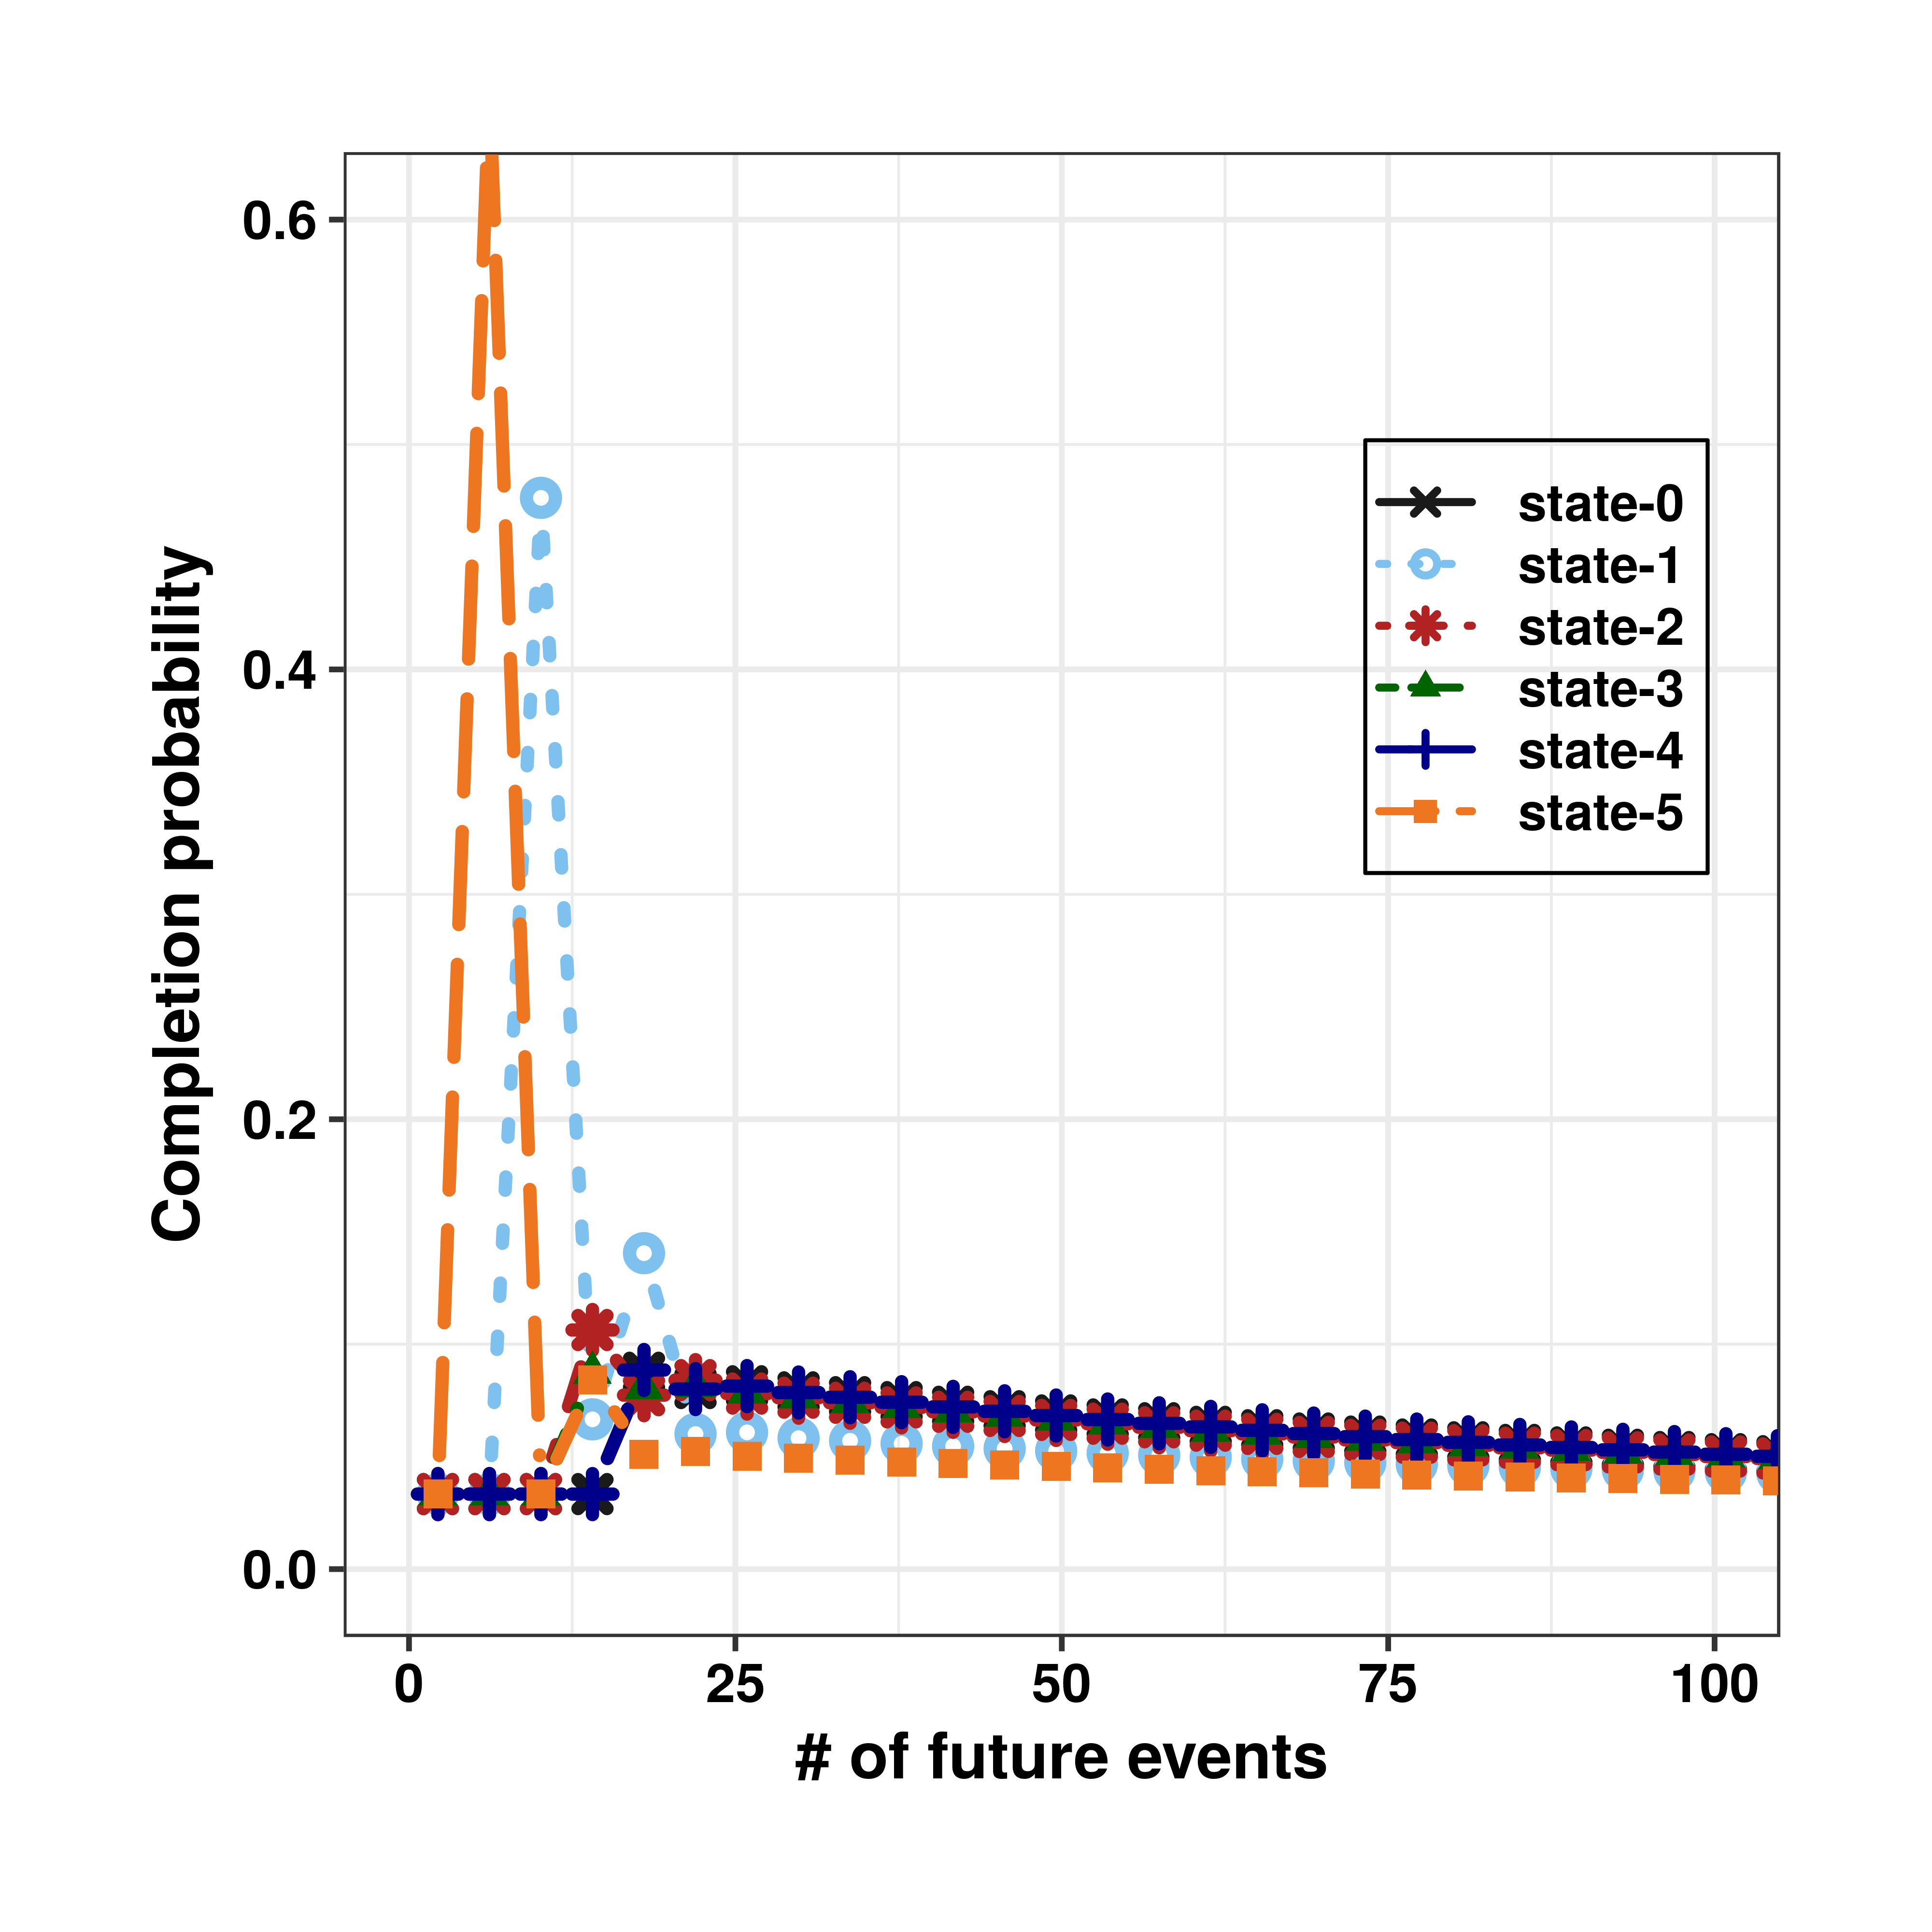
\includegraphics[width=.9\textwidth,height=.8\textheight]{../chapters/figures/new_wt.png}
			
			
			
		\end{centering}
	\end{figure}
	
	
}

\frame
{
	\frametitle{Event Forecasting with Pattern Markov
		Chains}
	\framesubtitle{Example of the computed prediction intervals for
		$\mathcal{P}=a ; d ; c$, $\Sigma=\{a,b,c,d\}$, $m=1$,$\theta_{p}=0.5,\ and\ \theta_{s}=20$.}
	
	\begin{figure}[]
		\begin{centering}
			\center
			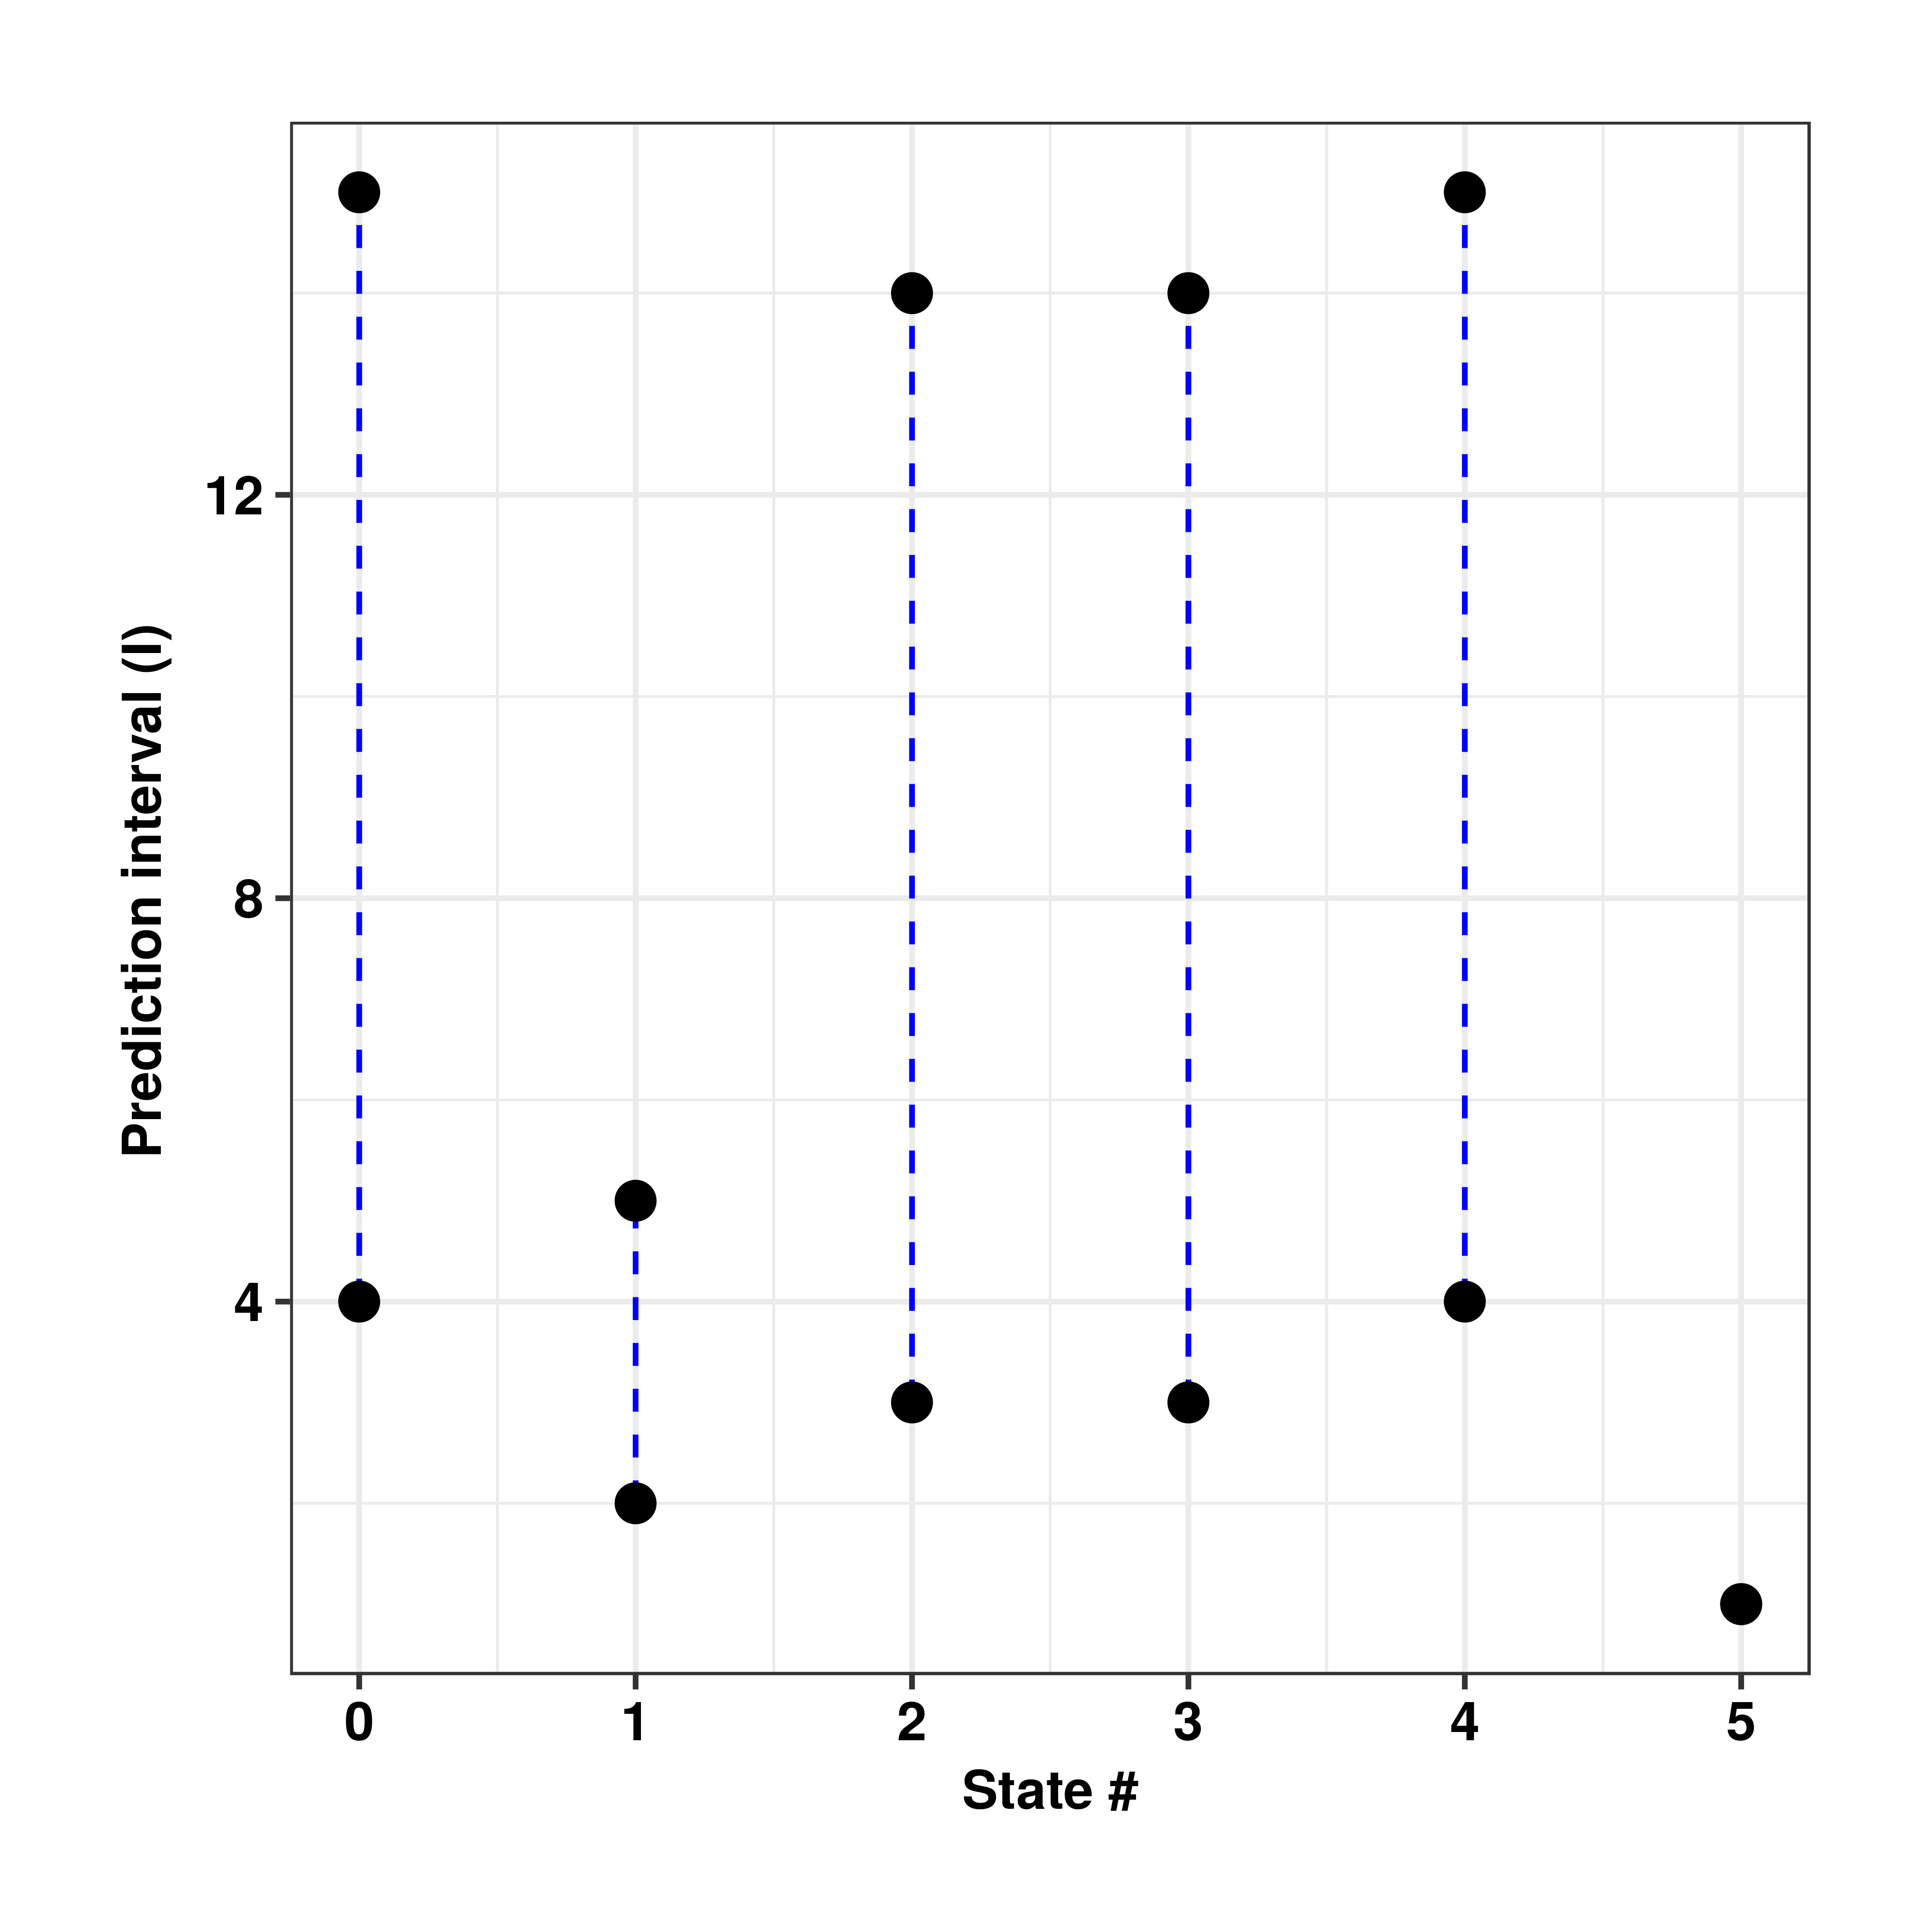
\includegraphics[width=.9\textwidth,height=.8\textheight]{../chapters/figures/new_prediction_intervals.png}
			
		\end{centering}
	\end{figure}
	
}


\frame
{
	\frametitle{Event Forecasting with Pattern Markov
		Chains}
	\framesubtitle{What is wrong?}
	\begin{itemize}
		
		\item<only@1> The overhead learning time of the Markov transition matrix for each input stream isolated from the others, how can we accelerate it?  
		 
		\item<only@1> The low performance of the model for an input event stream with less data. 
		
			\item<only@1> How can we enable the communication between the local models 
			 and leverage an aggregated global shared model in 
		 	a distributed and communication efficient fashion while maintaining
			provable and strong guarantees in service quality?
			
	
	\end{itemize}
}
